%
% include the class file for USI-INF Technical Reports
%
\documentclass{usiinftr}
\usepackage{float}
\usepackage{amsmath}
\usepackage{slashbox}
\usepackage{subfigure}
\usepackage{amsmath}
\let\circledS\undefined % here - PS
\usepackage{amssymb}
\usepackage{graphicx}
\usepackage{caption}
\def\code#1{\texttt{#1}}
\usepackage{newunicodechar} 
\DeclareUnicodeCharacter{FFFD}{?????}
\usepackage{hyperref} 
\DeclareMathOperator*{\argmax}{argmax}
\usepackage{multirow}
\usepackage{multicol}
\usepackage{pifont}

\begin{document}

\title{\bf Reproducibility challenge ATML SA 2021 \\ {\normalfont Generalization in Reinforcement Learning}}
\author{Erick Franciskus}{\ddagger}
\author{Glejdis Shk\"embi}{\ddagger}
\author{Constantin Jehn}{\ddagger}
\author{Jitin Jami}{\ddagger}

\affiliation{\dagger}{Faculty of Informatics, Universit\`a della Svizzera italiana, Switzerland}
\affiliation{\ddagger}{Faculty of Engineering, Friedrich-Alexander Universit\"at Erlangen-N\"urnberg, Germany}



%
% by default, the current month and year are used as the publication date
% of your Technical Report; if you want to change this, then you can do it here, e.g.
%
%\date{February~\the\year}
%\date{August 2011}

\maketitle
\begin{abstract}
Reinforcement learning (RL) is an important branch of artificial intelligence and is used in a variety of applications such as robotics, self-driving cars or solving complex board games like Go.
In contrast to supervised learning techniques, where evaluation is exclusively done on unknown data, classic RL algorithms are evaluated on the same environment it was trained on and generalization in RL remains an active branch of research.
We present a reproducibility study of a recent approach that was published by the Google Research Brain team under the title "Constrastive Behavioral Similarity Embeddings for Generalization in RL".
Our study includes a placement of the proposed approach in the field of generalization in RL, as well as a research on incorporated concepts.
Furthermore, we present the main benchmark environment and reproduce the main result from the paper.
We also study the model with respect to its sensitivity to hyperparameters and discuss other benchmark environments.


\end{abstract}

\section{Introduction}
Reinforcement Learning is used in sequential decision making for training agents in complex tasks. The agent interacts with the environment which, based on the agent's action, provides the agent with some reward (positive or negative). The agent then uses this feedback to update its behaviour with the goal of being optimal. Although current RL agents have demonstrated great potential in a variety of activities, they face difficulties in transferring these agent's capabilities to new unseen tasks. This happens even when the tasks are semantically equivalent. In other words, existing reinforcement learning agents frequently learn policies that do not generalize well to environments different than those environments these agents are trained on.

For example, the paper considers a jumping task, where we have an agent that needs to jump over an obstacle. The agent learns from image observations. In order for the agent to not collide with the obstacle, the agent needs to precisely time the jump at a particular distance from the obstacle. The various tasks consist of shifting the floor height or changing the obstacle position or both. If we train deep RL agents on some of these tasks where we vary the obstacle positions, they perform poorly at previously unseen locations (i.e. struggle to jump over the obstacle without hitting it). The challenge tackled in the paper is to generalize to unseen positions of the obstacle and floor heights in the test tasks, while using only a finite number of training tasks or environments sampled from a distribution of tasks.

\begin{figure}[h]
    \centering
    \begin{subfigure}
        \centering
        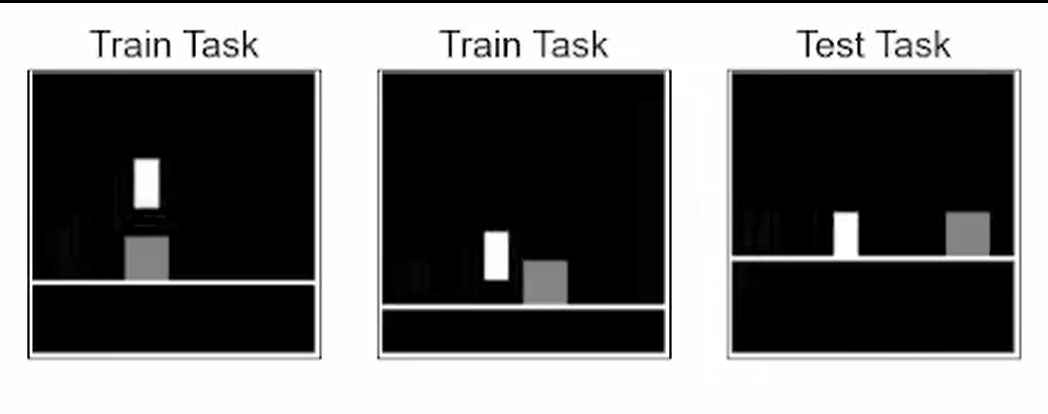
\includegraphics[width = 0.45\linewidth]{figures/image1.png}
        \label{}
    \end{subfigure}%
    \begin{subfigure}
        \centering
        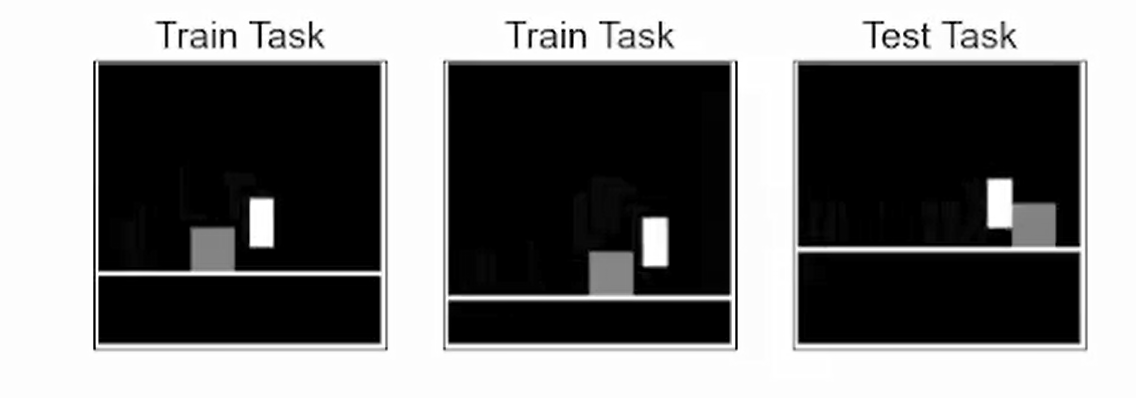
\includegraphics[width = 0.5\linewidth]{figures/image2.png}
        \label{}
    \end{subfigure}
    \caption{Train and Test task where agent fails}
    \label{fig:TrainTestTask}
\end{figure}

A few proposed solutions to poor generalization, adapted from supervised learning, include regularization (such as l2-regularization, dropout or noise injection), Domain Randomization and Data Augmentation (such as RandConv, RAD, DrQ), which is being used more recently. The majority of these ideas centre around improving the learning process in order to fully harness decision-making process, and they rarely use properties of the sequential aspect such as similarity in actions across temporal observations. Instead, this paper takes advantage of the fact that when an agent operates in similar tasks, the agent shows at least short sequences of behaviours that are similar across these tasks.

In their approach, the authors train the agents to learn a representation where the states are close when the optimal behaviour of the agent in the current states and future states are similar. They use the notion of behavioural similarity as it has the property of good generalization to observations across different tasks. This behavioural similarity between states across various tasks is quantified using the Policy Similarity Metric (PSM), which is a state-similarity metric based on bisimulation. Moreover, to enhance generalization, the agent is trained to learn state embeddings. This is done using Contrastive Similarity Metric (CSM).


\section{Theory and Concepts}

\subsection{Generalization in RL}
In supervised learning, training and test dataset are always held disjoint of each other.
And the performance of a predictor is generally evaluated on unseen test data.
In many RL benchmarks, like Atari, however the policy is evaluated on the same environment it was trained on and until now RL agents struggle to perform well on unseen environments \cite{lee2020network}.
Overcoming this limitation and making RL applicable to more realistic task is an active field of research.
Research on improving generalization in RL tries to produce "[...] algorithms whose policies have the desired
robustness, transfer and adaptation properties, challenging the basic assumption that train and test will be identical" \cite{kirk2021survey}.
\\
The type of generalization can be classified with respect to the distribution that training and test environments are drawn from: \cite{kirk2021survey}
\begin{itemize}
\item In singleton environments train and test environment are identical; no generalization is involved.
\item In i.i.d. generalization environments train and test environments are drawn from the same distribution: $P_{\text{train}} (C) = P_{\text{test}}(C)$.
\item The most challenging form of generalization are o.o.d generalization environments. Training and test environments are drawn from distinct distributions: $P_{\text{train}} (C) \neq P_{\text{test}}(C)$.
\end{itemize}
Furthermore, \cite{kirk2021survey} categorizes current research on generalization in RL.
The overview is shown in Figure \ref{fig: overview_research}. 
The branch "increasing similarity" aims to modify or augment the training environment to be similar to the training set.
"Handling differences" tries to address the difficulty that features will be different in the test environment. The paper we study tries to learn invariances: features that are not semantically important to the task should be discarded.
The first two groups could also be applied to supervised learning. The last branch aims to increase generalization by improving the optimisation on the training environment, which is specific to RL.

\begin{figure} 
\centering
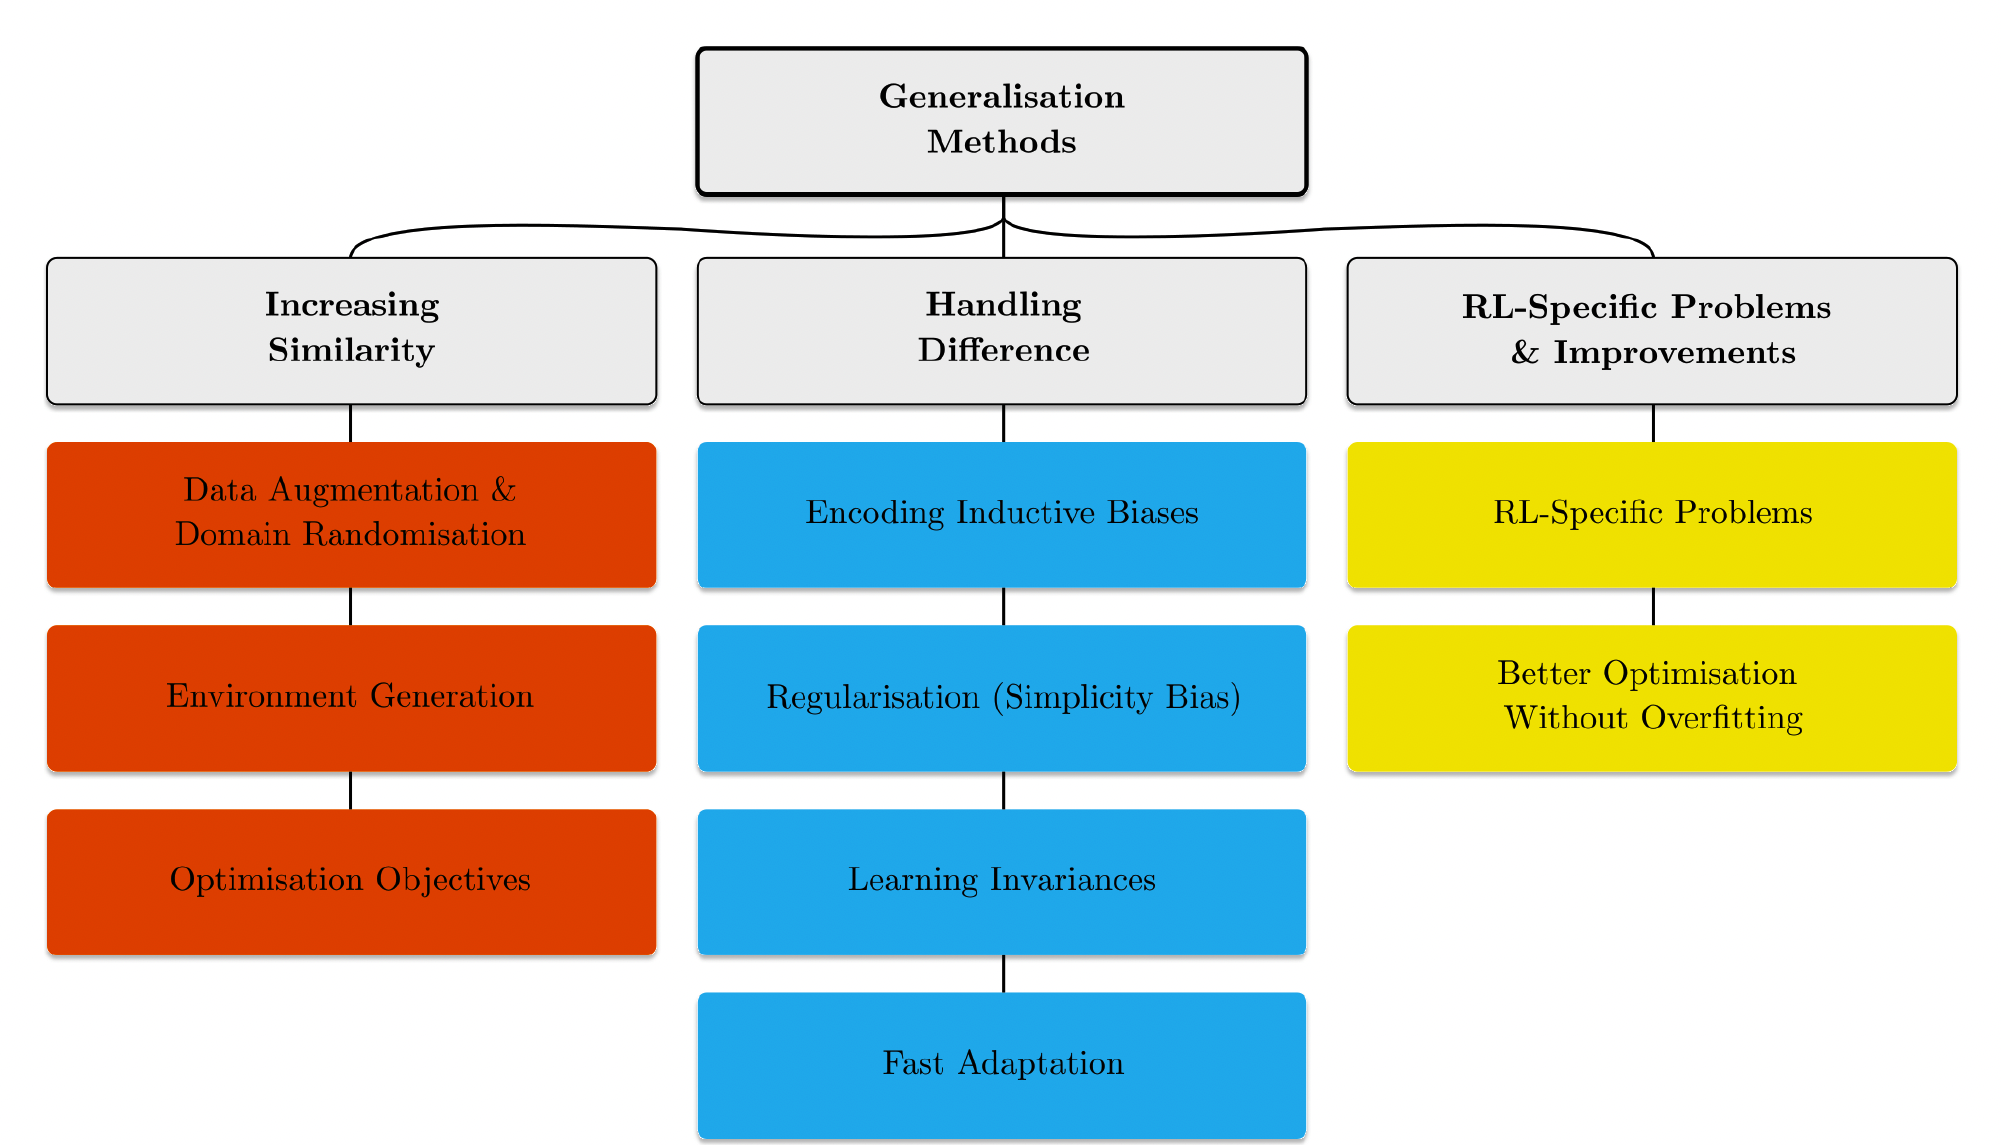
\includegraphics[width = 0.8\textwidth]{figures/Overview_research.png}
\caption{\label{fig: overview_research} Categorization of current research on generalization in RL according to \cite{kirk2021survey}. The studied paper \cite{agarwal2021contrastive} is an instance of learning invariances. }
\end{figure}

\subsection{State representation in RL} \label{sec: state repr}
Besides generalization, sample-efficiency is a major challenge in RL.
Learning successful policies from high-dimensional inputs like pixels of an image takes a huge amount of data.
Therefore, learning lower dimensional latent representations of environments is an active area of research in RL.
The agent then operates and learns policies in a latent space, which must be fully differentiable. \cite{hadeep}.
A useful representation, in the context of RL, would encode only task-relevant information of the original space.
There are well established dimensionality reduction methods like the Variational Auto-Encoder (VAE).
However, such methods assume all information of the input space to be important, which is not true for RL environments.
For instance, the task of jumping over block, depicted in Figure \ref{fig: optimal_trajectories}, is certainly invariant to the colour of the block.
Yet, this information would be encoded using a VAE, hindering generalization to the semantically identical task with a block of different colour.
Actively ignoring information that is irrelevant to the task is hence very desirable and can enhance generalization.
\cite{hadeep} \cite{kirk2021survey}
\subsection{The $\pi$-bisimulation and Policy Similarity Metric} \label{sec: PSM}
In the paper, the authors learn representations that encode behavioural similarity across states. To have a better understanding of the behavioural similarity, think of an agent who needs to reach spinach at the supermarket while maintaining social distancing of 6 feet. In the first environment to the left, the agent takes two actions to the right followed by two actions down. Now we look at the second environment on the right with a slightly different layout but where the agent takes the same actions (two steps right and two steps down) (as seen in figure \ref{fig:BehavioralSimilarity}). This is behavioural similarity where actions in the current state as well as in the future states are similar.

\begin{figure}[h]
    \centering
    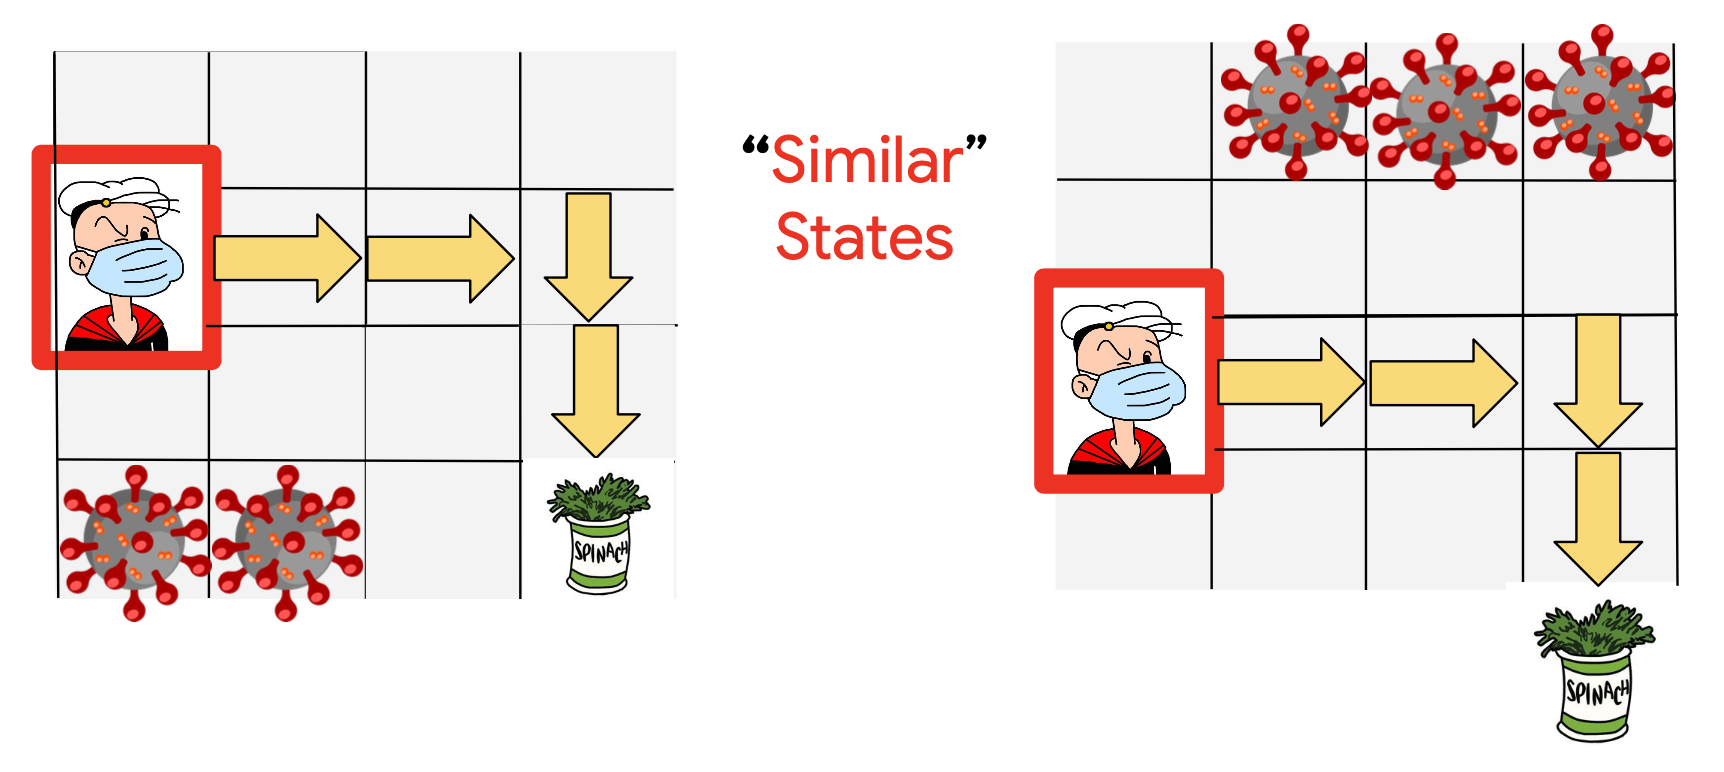
\includegraphics[width = 0.6\linewidth]{figures/image3.png}
    \caption{Understanding behavioral similarity. The agent needs to obtain the reward (spinach) while maintaining distance from the virus. Even though the initial states are visually different, they are similar in terms of their optimal behavior at current states as well as future states following the current state. Policy similarity metric (PSM) assigns high similarity to such behaviorally similar states and low similarity to dissimilar states.\cite{github_contrastive_similarity} }
    \label{fig:BehavioralSimilarity}
\end{figure}

To mathematically define the behavioural similarity, we use the concepts of bisimulation metric. Bisimulation metrics quantify the behavioural distance between two states in a Markov decision process. To mathematically define the bisimulation metric, we need some notations.

The Markov Decision Process (MDP) is defined as a 5-tuple M = (S, A, R, P, $\gamma$), where:
\begin{itemize}
    \item S denoted the set of all possible state.
    \item A denotes set of all possible actions.
    \item R denotes a reward function. $R(x,a,x')$ is the immediate reward received after $a$ transition from state $x$ to state $x'$ because of action $a$
    \item P denotes the state transition probabilities. $P(x,a,x')$ is the probability that action $a$ in state $x$ at time $t$ will lead to a state $x'$ at $t+1$.
    \item $\gamma \in  [0, 1)$  is the discount factor which is used to generate a discounted reward. \cite{puterman2005markov}
\end{itemize}

Each state $x$ encodes sufficient information about the environment such that an agent can learn how to behave in a consistent manner. Policy $\pi$ is a controller that helps us select the actions to maximize expected return $\mathbb{E}_{a_{t}\sim \pi(\cdot|x)} [\sum_t \gamma^t R(x_t,a_t)]$. A policy $\pi$(·$|$x) maps states $x \in X$ to distributions over actions. \\

In RL, the goal is to find an optimal policy $\pi^*$ that maximizes the cumulative expected return starting from an initial state $x_0$. In this paper, the goal is to learn a policy that generalizes well across related environments. \cite{agarwal2021contrastive}
 \\

An \textbf{equivalence relation}, $E \subset S \times S$, is a bisimulation relation if wherever 2 states, $(s,t) \in E$, are considered bisimilar (denoted $s \sim t$) if the following properties hold:

\begin{enumerate}
    \item They have equal immediate rewards: 
    \begin{itemize}
        \item $\forall a \in A, R(s,a) = R(t,a)$
    \end{itemize}
    \item Transition with equal probability to bisimulation equivalence classes:
    \begin{itemize}
        \item $\forall a \in A, \forall c \in S_E, P(s,a)(c) = \sum_{s'\in c} P(s,a)(s') = P(t,a)(c)$ \cite{castro2020scalable}
    \end{itemize}
\end{enumerate}

In other words, two states are bisimilar if they have similar expected rewards and dynamics. In the illustration (figure \ref{fig:BisimulationEquivalence}), we look at the system where a bisimualtion equivalence relation would collapse the 8 states on the left into an equivalent 4 state MDP to the right.

\begin{figure}[h]
    \centering
    \begin{subfigure}
        \centering
        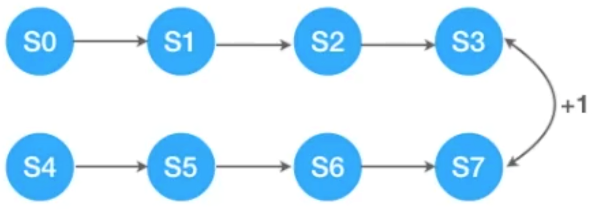
\includegraphics[width = 0.4\linewidth]{figures/image4.png}
        \label{}
    \end{subfigure}%
    \begin{subfigure}
        \centering
        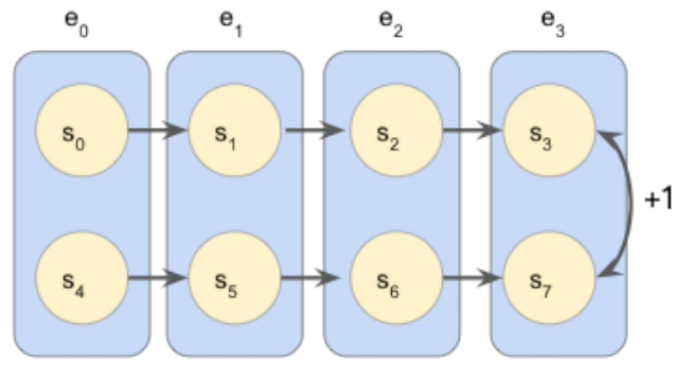
\includegraphics[width = 0.4\linewidth]{figures/image5.png}
        \label{}
    \end{subfigure}
    \caption{Bisimulation equivalence relation. The 8 states on the image on the left would collapse to an equivalent 4-states MDP \cite{pscsWebsite}}
    \label{fig:BisimulationEquivalence}
\end{figure}

Getting the exact equivalence would be quite tricky in every case, so we try to find a metric yielding a smoother notion of similarity than equivalence relation. The bisimulation metrics are a generalization of bisimualtion relations. Let $M$ be all pseudo-metrics of $S$, ie, all metrics $d \in M $ where $\forall (s,t) \in S, d(s,t)=0$. Define $F: M \rightarrow M$ to have a unique fixed point $d_{\sim}$, and this fixed point is a bisimulation metric:

\begin{equation}
    F(d)(s,a) = max_{a \in A} [|R(s,a) - R(t,a)| + \gamma \mathcal{W}_1 (d)(P(s,a),P(t,a))]
\end{equation}

where 
\begin{itemize}
    \item $s,t \in S$ are two states in the MDP.
    \item A is the action space.
    \item $R:S \times A \rightarrow R$ is the reward function.
    \item $P:S \times A \rightarrow \Delta(S)$ is the transition function.
    \item $\mathcal{W}_1 (d)$ is the Wasserstein distance between two probability distributions under a state metric $d$.
\end{itemize}
\cite{castro2020scalable}

A very nice theoretical property of such metric is that the bisimulation distance between two states is an upper-bound on their optimal value difference: $|V^*(s) - V^*(t)| \leq d \sim (s,t)$. \cite{castro2020scalable}

There are a few drawbacks of using reward difference in bisimulation for measuring state similarities:

\begin{enumerate}
    \item Two MDPs can have the same policies/behaviours but different expected rewards. For example, consider the two MDPs shown in figure \ref{fig:TwoMDP}. Once the agent has taken the action to eat cake, the agent should stop, because eating cake is good, but eating too much cake is bad. The rewards are different in these two MDPs. For certain values of these rewards, the bisimulation distance captures correct state similarity. \cite{slidelive}
\begin{figure}[h]
    \centering
    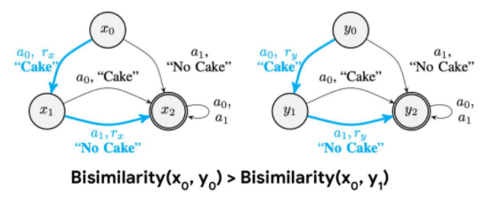
\includegraphics[width = 0.6\linewidth]{figures/image7.png}
    \caption{Same policies different rewards: Cyan edges represent optimal actions with a positive reward. The rest have zero reward. $x_0$, $y_0$ are the start states and $x_2$, $y_2$ denote the terminal states \cite{agarwal2021contrastive}}
    \label{fig:TwoMDP}
\end{figure}
    \item Two states can have the same long term expected reward but different optimal policies. For instance,  figure \ref{fig:ThreeJump} illustrates three jumping tasks with different positions of the obstacles. The three states with a yellow boundary have the same expected rewards, which means that the bisimulation value is 0. However, as illustrated with the little arrow, the optimal action in the first task in the highlighted is to jump, while in the other tasks the optimal action is to go right. 
\cite{slidelive}
\begin{figure}[h]
    \centering
    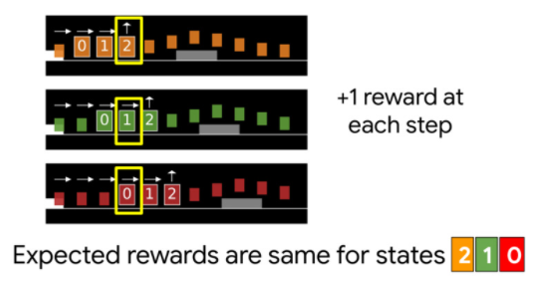
\includegraphics[width = 0.55\linewidth]{figures/image8.png}
    \caption{Same reward different policies: he three states with a yellow boundary have the same expected rewards, which means that the bisimulation value is 0. However, the exhibit different behaviour.  \cite{github_contrastive_similarity}}
    \label{fig:ThreeJump}
\end{figure}
    \item Pessimistic: the maximum is considering the worst possible case. \cite{castro2020scalable}
    \item Computational expense: Bisimulation metrics have been solved using dynamic programming, but as this requires updating the metric estimate for all state-action pairs at every iteration, it is computationally expensive. This means computing the Wasserstein distance $|S|\times|A|$ times at each iteration. \cite{castro2020scalable}
    \item Full state enumerability: Existing methods for computing/approximating bisimulation metrics require full state enumerability (countability). \cite{castro2020scalable}
    
\end{enumerate}

Therefore, to address these issues, in this paper, the $\pi$-bisimulation metric, which is based on the bisimulation metric, is being used. In contrast to bisimulation metrics, which is built on reward differences, $\pi$-bisimulation metrics are built on differences in optimal policies. they are called reward-agnostic. The pi-bisimulation metric is given by: \cite{castro2020scalable}

\begin{equation}\label{eq:BisimulationDistance}
    d_{\pi}(x,y) = |R^{\pi}(x) - R^{\pi}(x)| + \gamma \mathcal{W}_1(d_{\pi}) (P^{\pi}(\cdot | x), (P^{\pi}(\cdot | y)) 
\end{equation}


As it can be seen from equation \ref{eq:BisimulationDistance}, the bisimulation metric is a recursive equation with two terms. The first term calculates the reward difference, while the second term captures the long-term discounted future reward difference. Moreover, it defines the distance between two states x and y as the distance between expected rewards obtained when following policy $\pi$. The second term uses the Wasserstein-1 distance of the metric $d_{\pi}$. It quantifies the distance for the next state distributions following the policy $\pi$ at states x and y. A very easy illustration (\ref{fig:SandPile}) is to think of probability distributions as piles of sand. You can look at the sand pile as a probability mass. Then, the Wasserstein-1 distance calculates the dissimilarities between these piles of sand in terms of how much and how far we need to move the sand in order to transfer one pile into the other.

\begin{figure}[h]
    \centering
    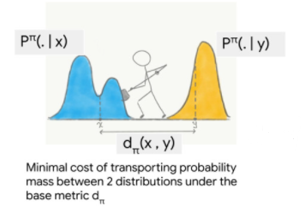
\includegraphics[width = 0.5\linewidth]{figures/image6.png}
    \caption{Sand Pile analogy of Wasserstein metric \cite{github_contrastive_similarity}}
    \label{fig:SandPile}
\end{figure}

The absolute reward differences are replaced by policy differences. Furthermore, as the goal is to perform well in previously unseen environments, we are interested in optimal behaviour, and so, we use $\pi^*$ as the grounding policy. This yields Policy Similarity Metric (PSM).

\begin{equation}
    d_{\pi}(x,y) = DIST(\pi^*(x), \pi^*(y)) + \gamma \mathcal{W}_1(d^*) (P^{\pi^*}(\cdot | x), (P^{\pi^*}(\cdot | y)) 
\end{equation}
\cite{castro2020scalable}


In PSM, states are considered similar when the optimal policies in these states as well as future states are similar. The DIST term captures the local optimal behaviour differences, while the Wasserstein term captures the long-term optimal behaviour differences. Moreover, the discount factor $\gamma$ assigns the weights. \cite{castro2020scalable}

Now, take into consideration transferring an optimal policy from one to another environment using PSM. We do this by finding the nearest neighbour x for each state y. This nearest neighbour has the minimum PSM distance to y. To define the transfer policy at y, the policy at x can be used. If we use this nearest neighbour transfer scheme, we have the advantage of an upper bound on the suboptimality of policies or optimal policies transferred from one environment to another by PSM, in contrast to bisimulation metric where we do not have such feature. 
\cite{castro2020scalable}
This illustrates how PSM provides a way of lifting generalization across inputs as a supervised learning problem to generalization across environments. As we aim to achieve a good generalization, we learn policy similarity embeddings that encode this PSM. This is done by adapting SimCLR, which is a constructive method for learning embeddings of image inputs.

\subsection{Policy Similarity Embeddings - PSEs}
Aiming for generalization of learned policies to related environments, the authors represent states in an embedding space, where closeness of states correlates with similar optimal policies. The embedding is built by self-supervised contrastive learning. Self-supervised learning refers to learning techniques that work without explicit annotations of the data. \cite{tian2021understanding} Instead, feedback signals are generated from the data itself. In this case this feedback comes from the policy similarity metric.   The contrastive instance of self-supervised learning works with positive pairs that are similar to each other, and negative or dissimilars pairs. \cite{Hadsell06dimensionalityreduction} The policy similarity metric d (introduced in Section \ref{sec: PSM}) is transformed to the similarity measure $\Gamma$ using the Gaussian kernel:
\begin{equation} \label{Gaussian Kernel}
\Gamma (x,y) = \exp ( -d(x,y)/ \beta) 
\end{equation}

For two state spaces $\chi' \subseteq \chi$ and $Y$ resulting from MDPs the positive pair $\{( \tilde{x}_y , y) \}$ is chosen as the one with highest similarity. Hence, $ \tilde{x}_y = \argmax_{x \in \chi'} \Gamma (x,y)$ , $y \in Y $.
All other states are grouped to negative pairs.
\\
Eventually, we aim to map unknown states into this embedding to infer successful policies. 
Therefore, a function $z_{\phi}(x)$ is needed that maps states into the embedding. 
The contrastive loss to learn this mapping is inspired from SimCLR, which also uses self supervised learning and heavy data augmentation to create a representation space of images that can be used for classification. \cite{chen2020simple}. The contrastive loss is given by: 

\begin{equation}\label{contrastive loss}
l_{\theta} (\tilde{x}_y, y; \chi' ) = 
- \log \frac{\Gamma (\tilde{x_y}, y ) \exp(\lambda s_{\theta} (\tilde{x}_y, y))}
{\Gamma(\tilde{x}_y, y) \exp (\lambda s_{\theta}(\tilde{x}_y, y)) + \sum_{x'\in \chi' \setminus \{\tilde{x}_y \}} (1 - \Gamma (x',y)) \exp (\lambda s_{\theta} (x',y))},
\end{equation}

where $s_\theta$ is the embedding similarity. The loss functions aims for a representation where positive pairs ($(\tilde{x_y}, y )$) have a high similarity in behaviour $\Gamma$ and in the embedding $s_\theta$ at the same time, corresponding to high value in the term (1) $\Gamma (\tilde{x_y}, y ) \exp(\lambda s_{\theta} (\tilde{x}_y, y))$.
On the contrary negative pairs ($x'\in \chi' \setminus \{\tilde{x}_y \}$) should be forced to be far from each other in the embedding space. So, small values in term (2) $\sum_{x'\in \chi' \setminus \{\tilde{x}_y \}} (1 - \Gamma (x',y)) \exp (\lambda s_{\theta} (x',y))$ are favourable.
Note that the whole loss is wrapped in a negative logarithm so small values of the argument lead to a high loss. The argument can take values in the range $(0,1)$.
High values in term (1) push the argument near 1 and leads to a "compensation" of values in term (2).
Low values in term (2) bring the argument closer to 1 and therefore a minimal loss.
\\
From here we can introduce the total contrastive loss for the MDPs $\mathcal{M}_\chi$ and $\mathcal{M}_y$. It uses the optimal trajectories $\tau_\chi^* = \{x_t\}_{t = 1}^N$ and $\tau_y^* = \{y_t\}_{t = 1}^N$.
$x_t$ and $y_t$ are the single states in the optimal trajectories. $x_{t+1}$ is the result of applying the optimal policy $\pi^*$ to transition dynamics $P$ of the system : $x_{t+1} \sim P_\chi^{\tau^*} (\cdot \mid x_t)$ and similar
$y_{t+1} \sim P_y^{\tau^*} (\cdot \mid y_t)$.
The authors set $\chi' = \tau_\chi^*$ (compare to Equation \ref{contrastive loss}) and then define the total contrastive loss as:

\begin{equation} \label{eq: total_loss}
L_\theta (\mathcal{M}_\chi, \mathcal{M}_y) = \mathbb{E}_{y \sim  \tau_y^*} [l_\theta (\tilde{x}_y, y;\tau_\chi^*)] . 
\end{equation}

$\tilde{x}$ is chosen as the most similar state to the given state y: $\tilde{x} = \argmax_{x \in \tau_\chi ^ *} \Gamma (x,y) $ . Then the loss between the Markov processes $\mathcal{M}_\chi$ and $\mathcal{M}_y$ are hence the expected value for y from the optimal trajectory of the contrastive loss (Equation  \ref{contrastive loss}) of $\tilde{x}$ and $y$ w.r.t. to the optimal trajectory of $x$.  The loss becomes low, if we can conclude states $\tilde{x}$ that are close w.r.t. its optimal trajectory from the similarity, in the representation space, to y. 


Figure \ref{fig: Learning_Architecture} gives an overview over the learning procedure as well as how inference is done.
An input pair (x,y) is fed in to the architecture.
First and optionally a data augmentation is applied: $\Psi_x := \Psi(x)$ and respectively $\Psi_y := \Psi(y)$.
Secondly the encoder $f_\theta$ is applied, which is the mapping we are in particular interested to train, $f_x = f_\theta (\Psi_x)$ and $f_y = f_\theta (\Psi_y)$.
The loss however is applied on a non-linear projection of the representation, $z_x = h_\theta(f_x)$ and $z_y = h_\theta(f_y)$, following the SimCLR approach \cite{chen2020simple}.
The inference of a suitable policy is done in the representation space $f_y$ as an affine function $\pi_\theta (\cdot \mid y) = W^T f_y + b$
with learnable parameters W and b.
The encoding learnt simultaneously during training of the agent, with auxiliary loss of Equation \ref{eq: total_loss}.

\begin{figure}[h]
\centering
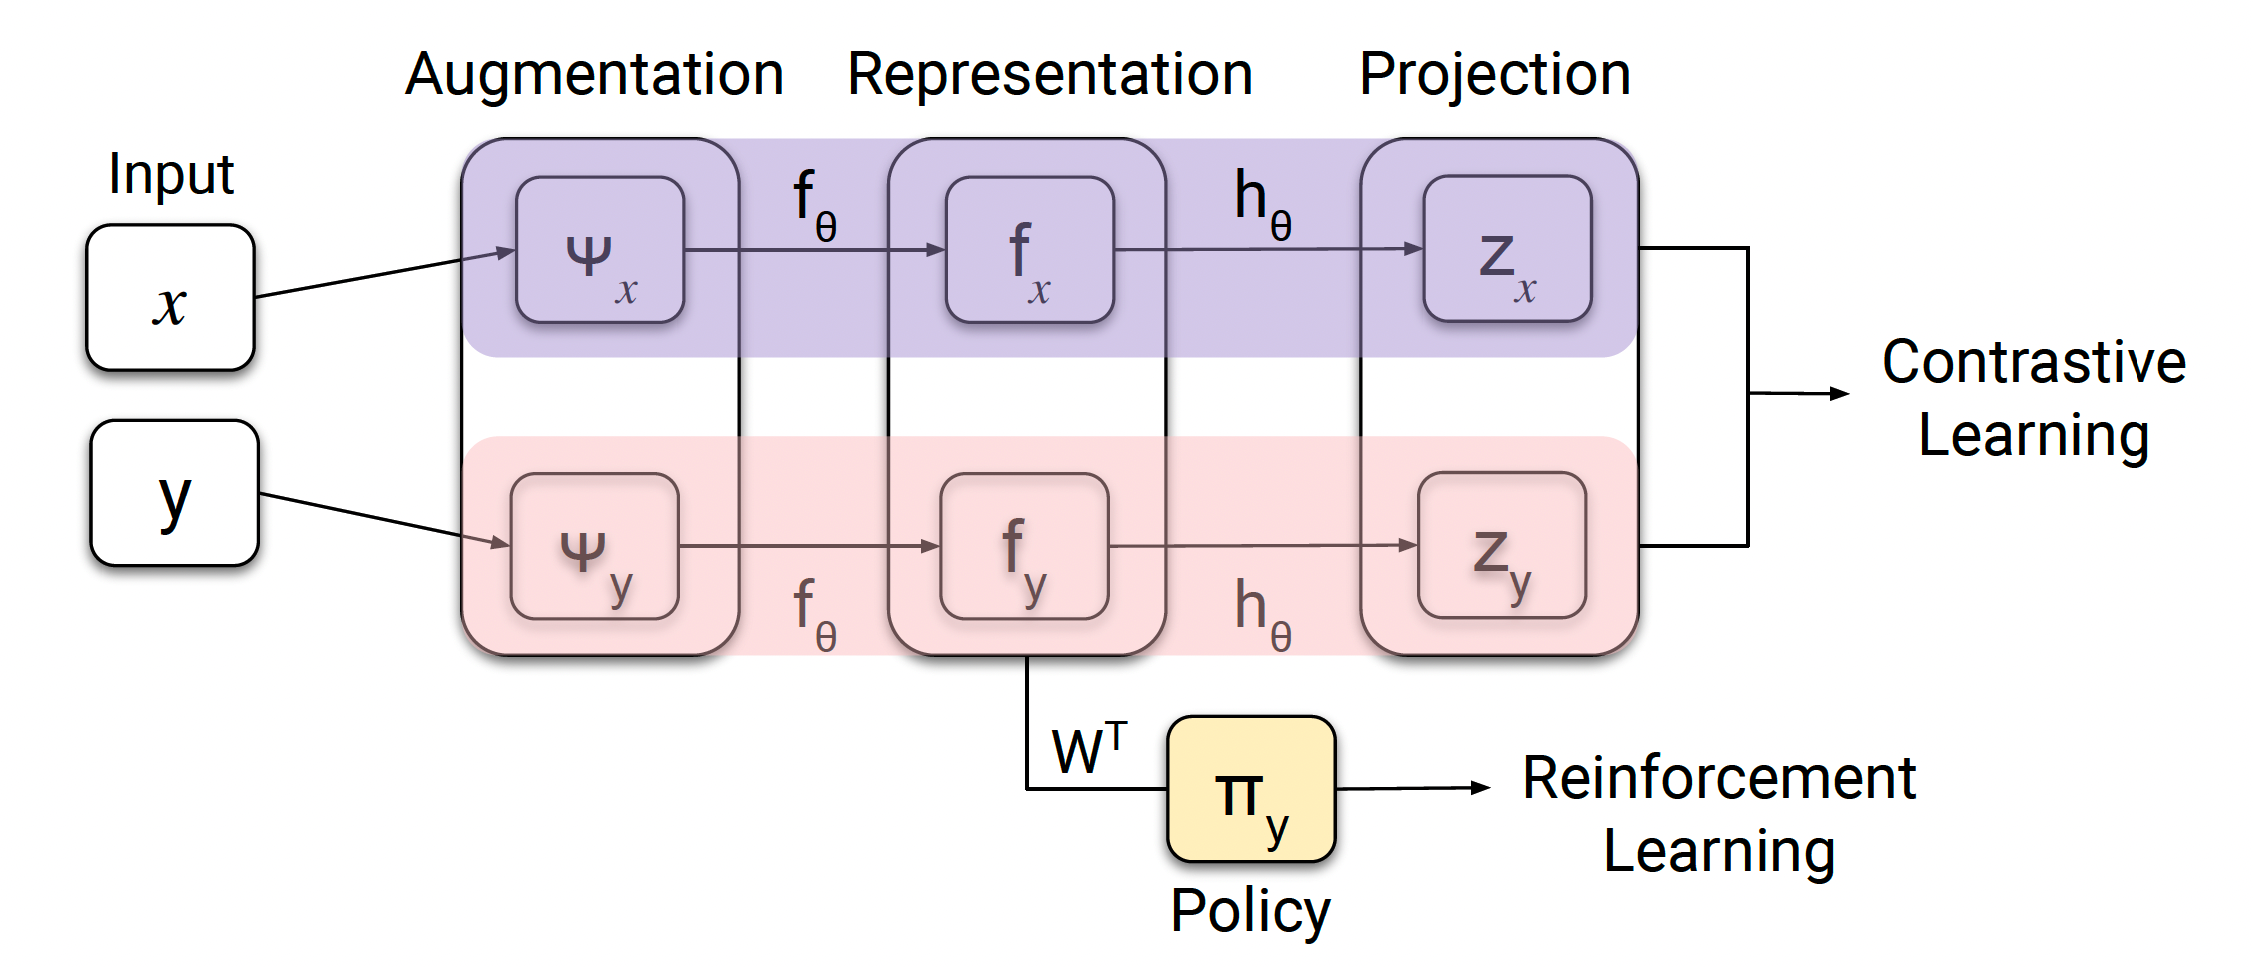
\includegraphics[width = 0.8\textwidth]{figures/Learning_architecture.png}
\caption{\label{fig: Learning_Architecture}An input pair (x,y) is first augmented and then mapped into the representation space $f$. The loss function defined in Equation \ref{eq: total_loss} is applied to a non-linear projection $z$ of this representation space. \cite{agarwal2021contrastive} }
\end{figure}


\section{Experiments from the paper}
In this section we want to introduce the paper's main experiment: the jumping task from pixels. The authors also studied generalization on the dm control suite where agents have to ignore visual distraction. However, we want to focus our reproducibility study on the jumping task.
\subsection{Jumping Task from Pixels: A Case Study}
In the jumping task, we have an agent that, learning from the image observations on pixel level, needs to jump over an obstacle. The agent can either go right or jump. To avoid a collision the agent needs to time the jump precisely. The environment can be adapted by changing the floor height and the position of the obstacle. Two possible environments and their optimal trajectory are shown in Figure \ref{fig: optimal_trajectories}. Generalization is reached, when the agent becomes invariant to such changes.
There are 26 different positions of the obstacle and 11 different values of the floor height. To stress generalization, the problem is split into 18 training tasks and the remaining 268 tasks are evaluation tasks.
\begin{figure}[h] 
\centering
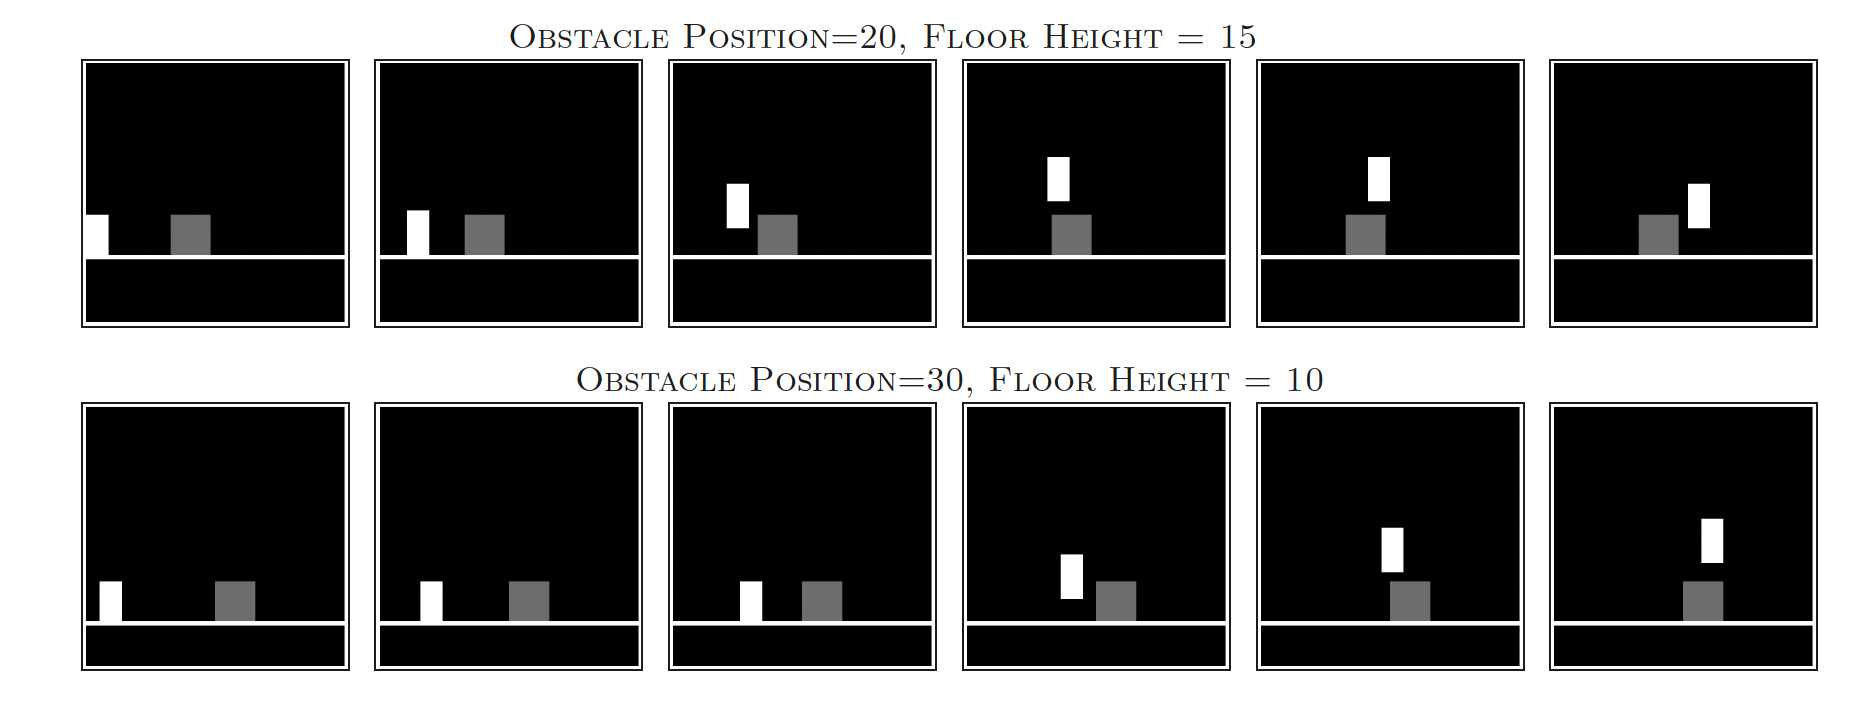
\includegraphics[width = 0.8\textwidth]{figures/optimal_trajectories.png}
\caption{\label{fig: optimal_trajectories}Optimal trajectories are shown for two different environments. The trajectory is a sequence of right actions interrupted by a single jump action. \cite{agarwal2021contrastive} }
\end{figure}


\subsection{Classification of the problem}
The states of the environment are discrete. This becomes apparent as we are able to classify all possible problems in a grid as combinations of obstacle position and floor height in Figure \ref{fig: grid_results}.
The actions of the agent are discrete as well: go right or jump.
The problem is deterministic because the optimal trajectory can be concluded with certainty.
In particular, by processing the fully observable input: all pixel values are available to the agent.
Furthermore, the problem is stationary because the optimal trajectory for a given task is time-invariant.
As the agent is the only active participant in the environment the problem can be considered a single agent task.
So the task actually falls into the "easiest" category of tasks for reinforcement learning. However, the aim of the authors is to study and improve generalization in RL. And the notion of generalization is very clear in this task and also measurable. Therefore, we think the task is very well chosen to study and show the ability of PSEs to improve generalization in RL.
\subsection{Results from the paper}
In the paper, three different grid configurations, that represent different styles of generalization are used:
\begin{itemize}
\item The wide grid tests generalization via interpolation
\item The narrow grid tests out-of-distribution generalization via extrapolation
\item The random grid evaluates generalization like supervised learning where the training and test samples are drawn i.i.d. (independently and identically distributed) 
\end{itemize}
All configurations are evaluated using the same hyperparameters that were tuned on the "wide" grid to show the robustness of PSEs to hyperparameter tuning. The authors compare the PSE to other regularization methods. 
Also the effect of data augmentation using RandConv is studied. RandConv is a recently proposed data augmentation method to improve generalization in RL. It uses a randomized convolutional neural network to perturb input observations randomly.
It aims to confront the agent with visually divers observations and hence mitigating overfitting to specific fix features in the input space. \cite{lee2020network}

\begin{figure}[h]
\centering
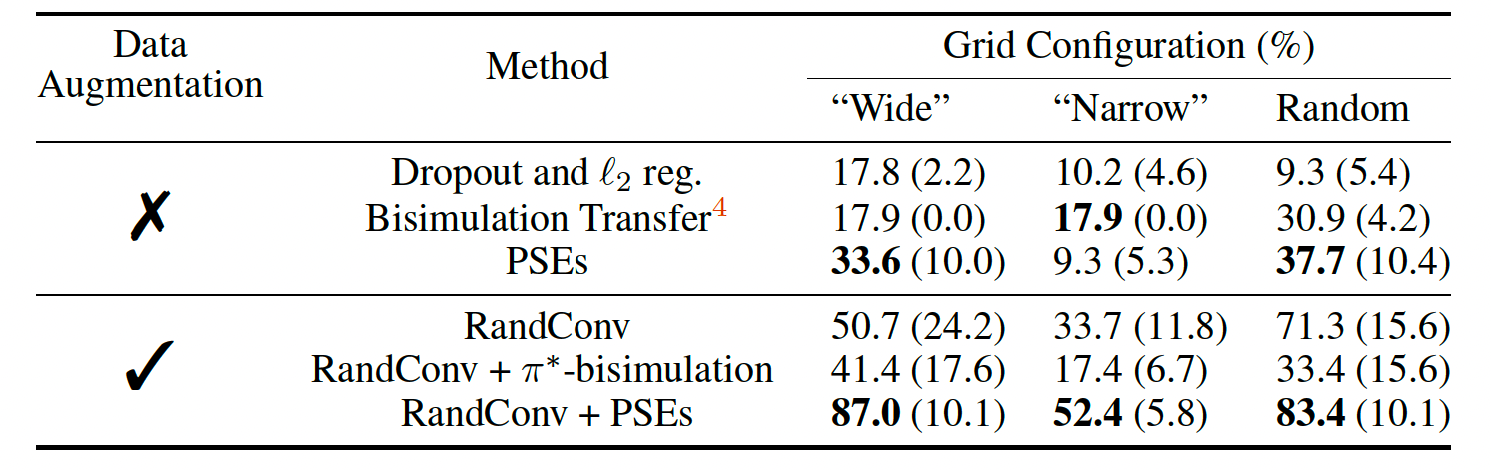
\includegraphics[width = 0.8\textwidth]{figures/tabular_results.png}
\caption{\label{fig: tabular_results}The table summarizes the main results of the authors, giving percentages of how many test tasks could be solved using different methods with or without data augmentation. The grid configurations are shown in Figure \ref{fig: grid_results}. It can be observed that PSEs outperform the compared methods in most configurations except for the narrow grid without data augmentation.
Also, PSEs profit substantially from data augmentation. \cite{agarwal2021contrastive}}
\end{figure}

The average performance across 100 runs is reported in Figure \ref{fig: tabular_results}. 
PSEs outperform all other methods except for the case without data augmentation on the narrow grid. It is also apparent that PSEs work particularly well with data augmentation.
The different grid types as well as the performance of PSEs + data augmentation are shown in Figure \ref{fig: grid_results}.

\begin{figure}[h] 
\centering
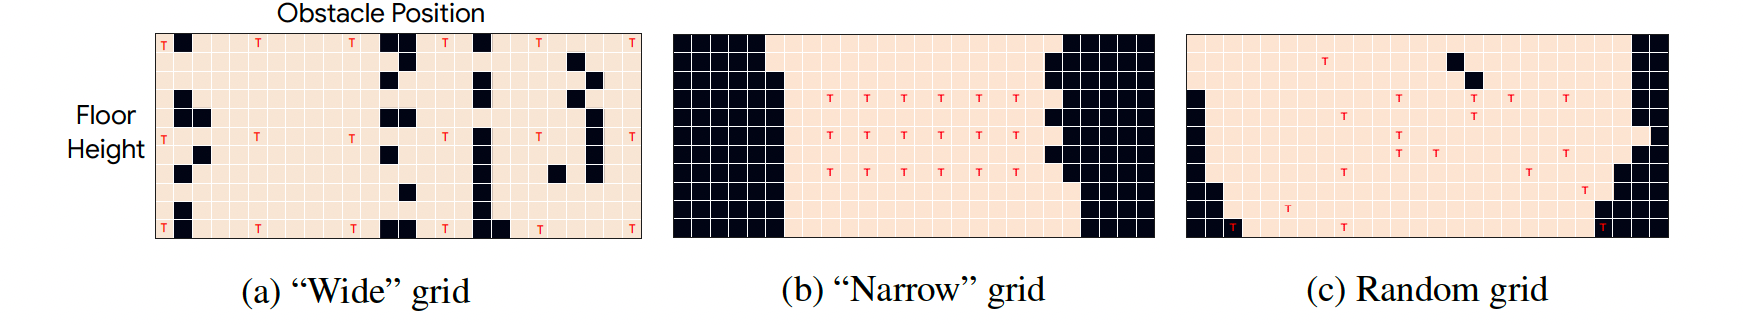
\includegraphics[width = 1\textwidth]{figures/grid_results.png}
\caption{\label{fig: grid_results}The red letter T shows which are the training tasks for the three grid configurations and the background colour of each tile shows the performance of PSEs across the task configurations, which is reported as the median of 100 runs per configurations using data augmentation. Beige tiles correspond to tasks that could be solved and black tiles could not be solved. \cite{agarwal2021contrastive}}
\end{figure}

\section{Results of reproducibility study}
In this section, we elaborate on how we attempted to reproduce the results that were presented in the paper. The authors of this paper published their codes for both the jumping task from pixels task and the distracting control suite tasks with 6 different environments. We discuss in detail the reproducibility of these tasks and the corresponding results from these experiments.

\subsection{Jumping Task from Pixels : Main result}
In the jumping task code, the authors generate imitation learning dataset from a certain hardcoded ideal policy of the pixel jumping task game itself, whereby the action jump would be selected only when the agent state is at a certain horizontal distance away from the obstacle. Otherwise the ideal policy would always maintain a "go right" action for the agent. Referring to the scheme described by the authors in figure \ref{fig: Learning_Architecture}, the states of the agent from this ideal policy are the x inputs and the actions of agent from this ideal policy are the y inputs. These inputs are then augmented and projected before being fed into an adapted Nature DQN. During training with the training environment grid, the model would then learn ideal policies, which are iteratively evaluated against evaluation jumping task environments. These are done until a certain number of training epochs is achieved. The author set the default training epoch as 2000 epochs. The results for the different augmentation, embedding and loss function ablation configurations are then averaged over 100 runs as summarized in Figure \ref{fig: tabular_results}.

The code itself is well structured and relatively reproducible. We encountered minor difficulty setting up the framework due to the discrepancies between the required packages versions as specified in their requirements.txt file and the machines where we run our experiments on. However, this did not significantly hinder us from running the code. The custom written gym based jumping task environment was also relatively simple to register and use. Changing the hyperparameters, training grid width and the different augmentation, embedding and loss function options is also very intuitive as one only needs to modify the command line option flags when running the main training script. For each run, the logs of various metrics such as number of tasks solved, loss and solved plots are saved within tensorboard logs. This also allows us to obtain the experiment results and visualize them easily. 

When the script is run from our local PC CPUs, each training run of 2000 epochs takes in average about 2 hours to complete. The code provides GPU acceleration possibilities. When the script is run from a HPC cluster with an Intel Xeon CPU E5-26802 with four corse and two NVIDIA P100 GPUs, each training run of 2000 epochs takes in average about 50 minutes to complete. Therefore, this jumping task experiment itself may not be very easy to reproduce for those who do not have access to ample computing power.

Due to time and computing power allocation in the HPC cluster constraints, we reduce the number of training runs from 100 runs to 5 runs. The hyperparameters, training grid width settings and ablation parameters are set according to the instruction given by the author in the readme of the Git repository. The results of the jumping task study with different training grid width and ablation parameters are summarized in the following table.


Additionally, for visualization purposes, we have also obtained the training log plots and the training grid visualizations that we can compare with the figures found within the paper.

Talk about our result vs publication.
\begin{figure}[h]
    \centering
    \begin{subfigure}
        \centering
        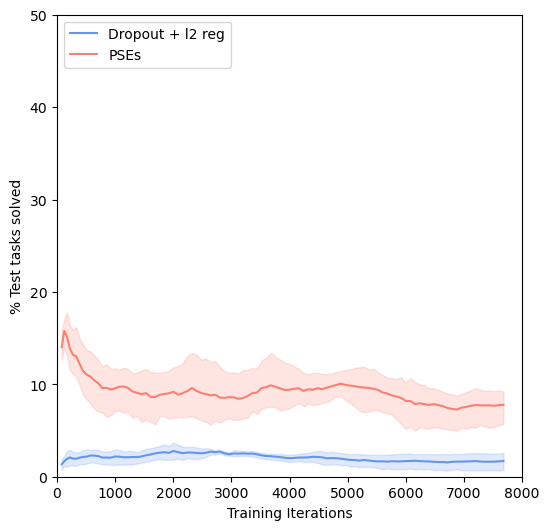
\includegraphics[width = 0.3\linewidth]{figures/narrow_without_data_aug.png}
        \label{}
    \end{subfigure}%
    \begin{subfigure}
        \centering
        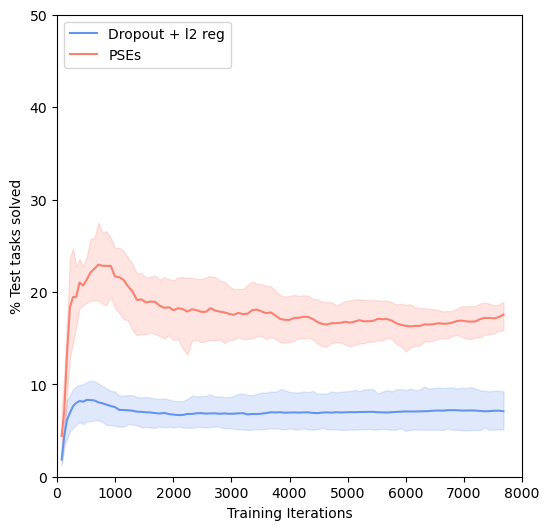
\includegraphics[width = 0.3\linewidth]{figures/wide_without_data_aug.png}
        \label{}
    \end{subfigure}%
    \begin{subfigure}
        \centering
        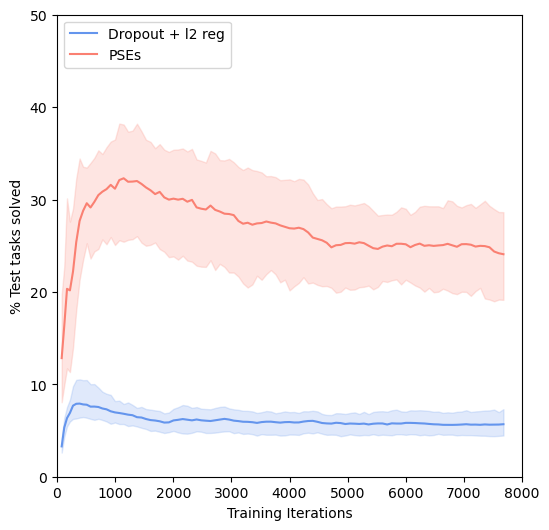
\includegraphics[width = 0.3\linewidth]{figures/random_without_data_aug.png}
        \label{}
    \end{subfigure}%
    \caption{Test performance curves in the setting \textbf{without data augmentation} on the wide, narrow, and random grids. We plot the median performance across 5 runs. Shaded regions show 25 and 75 percentiles}
    \label{fig:ResultWithoutDataAug}
\end{figure}

\begin{figure}[h]
    \centering
    \begin{subfigure}
        \centering
        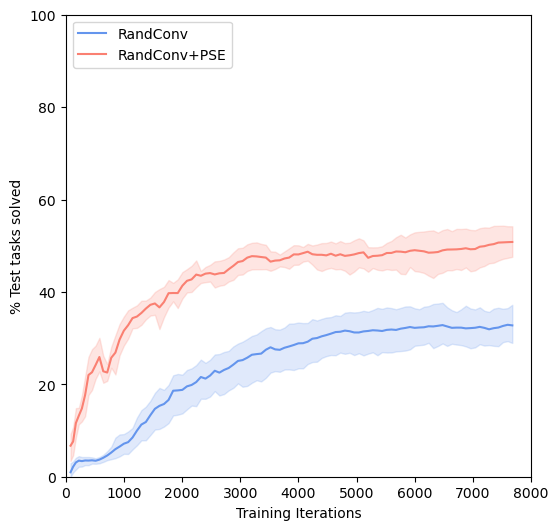
\includegraphics[width = 0.3\linewidth]{figures/narrow_with_data_aug.png}
        \label{}
    \end{subfigure}%
    \begin{subfigure}
        \centering
        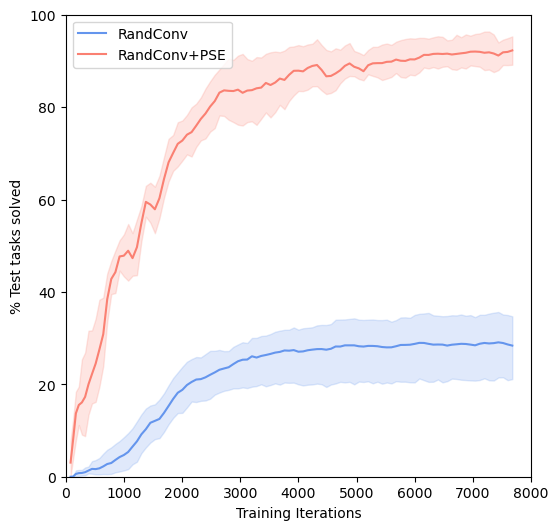
\includegraphics[width = 0.3\linewidth]{figures/wide_with_data_aug.png}
        \label{}
    \end{subfigure}%
    \begin{subfigure}
        \centering
        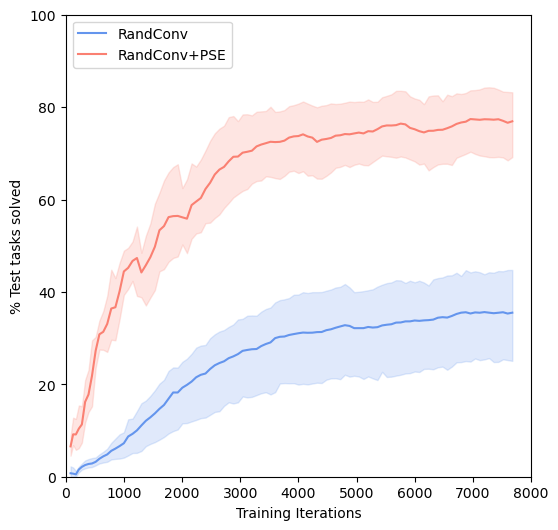
\includegraphics[width = 0.3\linewidth]{figures/random_with_data_aug.png}
        \label{}
    \end{subfigure}%
    \caption{Test performance curves in the setting \textbf{with data augmentation} on the wide, narrow, and random grids. We plot the median performance across 5 runs. Shaded regions show 25 and 75 percentiles}
    \label{fig:ResultWithDataAug}
\end{figure}

\begin{table}[h]
\caption{Percentage (\%) of test tasks solved by different methods without and with data augmentation. The wide, narrow, and random grids. We report average performance across 5 runs with different random initializations, with standard deviation between parentheses}
  \centering
  \renewcommand{\arraystretch}{1.2}
  \begin{tabular}{c*{3}{c}{c}} \hline
    \multirow{2}{*}{Data Augmentation} & \multirow{2}{*}{Method} & \multicolumn{3}{c}{Grid Configuration (\%)}\\
    \cline{3-5} & & Wide & Narrow & Random\\
    \hline
    \multirow{3}{*}{\ding{55}} & Dropout and $l_2$ reg & 6.86(2.27) & 1.86(1.05) & 5.82(1.64)\\
     & Bisimulation Transfer & 17.91(0.23) & \textbf{14.55}(1.33) & 14.77(3.96)\\
     &  PSEs & \textbf{18.58}(2.35) & 7.91(1.25) & \textbf{23.65}(5.95)\\
    \hline
    \multirow{3}{*}{\ding{51}} & RandConv & 27.38(7.95) & 32.23(5.04) & 36.26(10.43)\\
     & RandConv + $\pi^*$-bisimulation & 18.35(0.72) & 28.58(14.13) & 29.62(13.58)\\
     & RandConv + PSEs & \textbf{93.58}(4.01) & \textbf{50.97}(3.05) & \textbf{78.20}(8.08)\\
    \hline
  \end{tabular}
  \label{table:Rec_bisection}
\end{table}


\subsection{Jumping Task from Pixels : Hyperparameter Sensitivity tests}
The default hyperparameters used by the author for the jumping taks pixels are summarized in the following table. 

These hyperparameters were obtained from validation experiments done by the author with wide grid training grids, random convolutions and PSE loss, whereby the chosen values result to the best possible performance of the agent in that specific setting. We are interested in investigating the sensitivity of four of the hyperparameters used, namely learning rate, temperature, soft-coupling temperature, and $\alpha$. We set a 5\% decrease and increase to each one of these four hyperparameter values while keeping the remaining hyperparameters as the default chosen values. We then compare the performance, which in this case is the number of tasks solved, with the default wide grid result obtained from the previous subsection. Due to time and computing power allocation in the HPC cluster constraints, each hyperparameter sensitivity test is done in 3 runs. The overall sumamry of the effect of each hyperparameter to the performance of the agent is summarized in the following table.


\subsection{DM Control Tasks}
The author also published their code for DM Control Tasks, whereby the generalization ability of PSE are tested with 6 different environments with continuous states and actions, namely Ball in Cup Catch, Cartpole+Swingup, Cheetah-Run, Finger-Spin, Reacher-Easy, and Walker-Walk. The model are trained in environments with 2 different video distractions obtained from DAVIS dataset playing in the background and then evaluated against environments with 30 other video distractions from DAVIS dataset in the background. The author utilizes Soft Actor Critic Network with clipped double-Q network for the actor network. The loss term combines four loss terms, namely actor loss, critic loss, temperature loss, and PSE loss. Optimal policies are approximated by policies from each environment obtained after 500000 iteration steps. 

Reproducing the DM Control Task was significantly more intricate compared to the jumping task. First of all, the video distraction used in this test requires both distraction\_control and dm\_control infrastructure packages, which were both specially developed by Deepmind. These 2 packages requires an additional UC Davis images and videos database folder which needs to be separately downloaded into the local machine. Additionally, these packages also require an installation of MuJoco, which is the Deepmind multiphysics simulation infrastructure. While the installation steps of these frameworks are specified within the repositories of each of these packages, there were still multiple separate components which needed to be installed and configured separately. Furthermore, some of the requirements.txt given in the repositories point to deprecated versions of Python packages, which also result to conflicts and errors while attempting to set up this environment. While these conflicts could still be solved, this still significantly hinders the setting up process of this task. 

Secondly, the soft actor critic network requires an action replay buffer. In the code written by the authors, they utilize tf-agents with an experimental Tensorflow specific action replay buffer developed by Deepmind called reverb. This was not possible to install in our local machines as this reverb action replay buffer framework is currently only supported in Linux OS and not in Windows or Mac OS, as indicated in the repository of the reverb package. This is not specified at all in the dm control tasks code repository. Therefore, it was not possible for us to reproduce the dm control tasks at all.  
\subsection{Different Environment Tests}
It would also be interesting to test the generalization ability of PSE with different environments. While this was already done within the DM control tasks with 6 different environments, it is currently not reproducible due to the aforementioned issues. However, one of the biggest issue of testing a different environment is obtaining the optimal policy for the imitation learning process. For the jumping task problem, the optimal policy was easily hardcoded due to the sheer simplicity of the jumping task itself. However, such an optimal policy cannot be easily obtained in many different common RL test environments. While this could also be approximated with policies obtained from a very high number of iterations as obtained in the DM Control Tasks, it may also be unrealistic to approximate policies as such with limited computing resources and time. As such, we come to the conclusion that testing PSE with different environments and setup may not be feasible at the moment. 
\subsection{Overall Remarks Regarding Reproducibility}
\subsection{Workload Partition among Group Members}
Constantin and Glejdis worked mostly on the theoretical part of the report, by providing a thorough examination on the methods used and the mathematical explanations behind it, and provided the results from the original paper. While Glejdis focused more on behavioural similarity, the $\pi$-bisimualtion and Policy Similarity Metric, Constantin analysed Generalization and State Representation in RL, and Policy Similairty Embeddings. \\
Jitin has worked on the report with Glejdis on the parts about the $\pi$-bisimualtion and Policy Similarity Metric. He has worked on running the code for some of the various methods and different placements with Erick. He has also worked on visualization of results as well as ensuring report quality as a blind reviewer in the end.\\
\bibliographystyle{plain}
\bibliography{citations}

\end{document}
